\documentclass[10pt,a4paper]{article}

%%%%%%%%%%%%%%%%%%%%%%%%%%%
% MODIFY:

\newcommand{\authorA}{Thomas Mustermann (1234567890)}
\newcommand{\authorB}{Maria Musterfrau (1234567891)}
\newcommand{\authorC}{Alexander Musterstudent (1234567892)}
\newcommand{\groupNumber}{123} % - YOUR GROUP NUMBER
\newcommand{\exerciseNumber}{1} % - THE NUMBER OF THE EXERCISE
\newcommand{\sourceCodeLink}{https://www.github.com/link/to/our/github/project}

\newcommand{\workPerAuthor}{
\authorA&Task 1&0\%\\
      &Task 2&20\%\\
      &Task 3&30\%\\
      \hline
\authorB&Task 1&100\%\\
      &Task 2&40\%\\
      &Task 3&30\%\\
      \hline
\authorC&Task 1&0\%\\
      &Task 2&40\%\\
      &Task 3&40\%
}

%%%%%%%%%%%%%%%%%%%%%%%%%%%

%%
% imports for the exercise sheets
%

\usepackage[utf8]{inputenc}
\usepackage{amsmath}
\usepackage{amsfonts}
\usepackage{amssymb}

\usepackage[yyyymmdd]{datetime}
\renewcommand{\dateseparator}{--}

\usepackage[left=2cm,right=2cm,top=3cm,bottom=3cm]{geometry}

\usepackage{hyperref}

\usepackage{amsthm}
\newtheorem{lem}{Lemma}
\newtheorem{thm}{Theorem}
\newtheorem{cor}{Corollary}
\newtheorem{rem}{Remark}
\newtheorem{definition}{Definition}
\newtheorem{ter}{Terminology}

\usepackage{graphicx}

\newcommand{\M}{\mathcal{M}}
\newcommand{\N}{\mathcal{N}}
\newcommand{\K}{\mathcal{K}}
\newcommand{\SPDk}{\mathbb{P}^k}
\newcommand{\vol}{\text{vol}}

\newcommand{\Figref}[1]{Figure~\ref{#1}}
\newcommand{\figref}[1]{figure~\ref{#1}}
\newcommand{\Eqnref}[1]{Equation~(\eqref{#1})}
\newcommand{\eqnref}[1]{equation~(\eqref{#1})}

\usepackage{float}
\usepackage{tabularx}
\usepackage{subcaption}
\usepackage{mwe}

\usepackage{fancyhdr}
\pagestyle{fancy}

\usepackage{totcount}
\newtotcounter{taskCounter}
\newtotcounter{pointCounter}
\newenvironment{task}[1]{\noindent\stepcounter{taskCounter}\textbf{Report on task #1}\smallbreak\hrule\smallbreak}{\smallbreak\hrule\bigbreak}


\title{Report for exercise \exerciseNumber~from group~\groupNumber}

\makeatletter
\let\thetitle\@title
\let\theauthor\@author
\let\thedate\@date
\makeatother

\providecommand{\versiondate}{\today}

\lhead{Exercise sheet \exerciseNumber}
\chead{Master Praktikum: Modelling and Simulation of Crowds WS2019/20}
\rhead{TUM}
\lfoot{Report of Group \groupNumber}
\cfoot{\thepage}
\rfoot{Last compiled: \versiondate}
\renewcommand{\headrulewidth}{0.4pt}
\renewcommand{\footrulewidth}{0.4pt}

\newcommand{\frontpage}{
\begin{center}
\textbf{\thetitle}\\~\\
\end{center}
\begin{table}[H]
\begin{tabular}{ll}
Tasks addressed:&\total{taskCounter}\\
Authors:&\authorA\\
&\authorB\\
&\authorC\\
Last compiled:&\versiondate\\
Source code:&\sourceCodeLink
\end{tabular}
\end{table}
\vfill
The work on tasks was divided in the following way:
\begin{table}[H]
\begin{tabularx}{\textwidth}{X|p{2cm}|p{2cm}}
\workPerAuthor
\end{tabularx}
\end{table}
\newpage
}

\begin{document}

\frontpage

\begin{task}{1, Setting up the Vadere environment}
We successfully downloaded the vadere software and ran it. We simulated the RiMEA scenarios 1 (straight line) and 6 (corner) as well as the "chicken test". For all of these simulations we used the Optimal Steps Model (OSM).
In the following paragraph we compare the vadere simulation of  these scenarios with our own cellular automoton simulation of the first exercise.
\begin{itemize}
    \item RiMEA scenario 1 (straight line): \\
    We set up the vadere simulation of the first RiMEA scenario with a mean speed of 1.33, a minimum speed of 1.25 and a maximum speed of 1.44. Moreover we set up the speed standard deviation to 0.1.
    The pedestrian took with 29.999 seconds almost 30 seconds. This is very close to our result we achieved with our own implemented cellular automoton in the first exercise (29.67s). One  difference of vadere to our simulation is that the RiMEA scenarios are already set up so we only configured the speed, but the setup of the topography was already done. Moreover the pedestrian in our cellular automoton walks straight because we use cells with a shape of a rectangular. In the vadere simulation the pedestrian walks a little bit up and down. We think that the reason for this behaviour is that the grid consists of hexagonal cells. So the resolution of the grid is very high. In Figure \ref{fig:rimea1_osm} you can see the simulated scenario and recognize how the pedestrian walked up and down and not totally straight to the target.
     \begin{figure}[H]
        \centering
        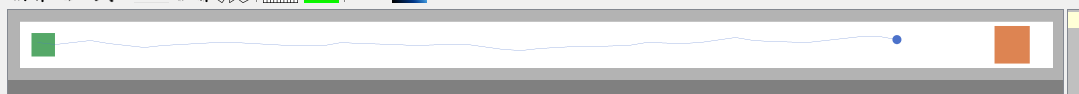
\includegraphics[width=0.7\textwidth]{pictures/osm/rimeatest1.png}
        \caption{RiMEA Scenario 1 with OSM}
        \label{fig:rimea1_osm}
    \end{figure}
    \item RiMEA Scenario 6 (corner):\\
    We set up the RiMEA scenario 6 with a mean speed of 1.34. Moreover we set the minimum speed to 0.5 and the maximal speed ot 2.2. The speed standard deviation was set to 0.26. We choose the RiMEA scenario from a list of pre-defined scenarios which vadere offers. So we didn't need to set up the topography by ourselves. The following table shows for every pedestrian the evacuation time.
    \bigbreak
    \begin{tabular}{c|c}
    pedestrianID& evacuationTime\\
    \hline
    1& 16.8  \\
    2& 19.2 \\
    3& 21.2\\
    4&17.2\\
    5&20.0\\
    6&10.4\\
    7&24.4\\
    8&20.2\\
    9&20.8\\
    10&24.0\\
    11&17.6\\
    12&33.2\\
    13&16.8\\
    14&14.0\\
    15&12.8\\
    16&27.2\\
    17&20.4\\
    18&25.6\\
    19&11.2\\
    20&15.6\\
    \end{tabular}
    \bigbreak
    In comparison to our simulation from the first exercise we did not record the time every pedestrian needs to reach the target. We recorded only the time that all pedestrians took to reach the target around the corner. Furthermore vadere shows the single paths of the pedestrians to the target, while in our cellular automoton it was only possible to see which cells were not part of any path to the target. Figure \ref{fig:rimea6_osm} shows the RiMEA 6 sceanrio simulated with the Optimal Steps Model. The picture shows which path the single pedestrians take to reach the target.
    \begin{figure}[H]
        \centering
        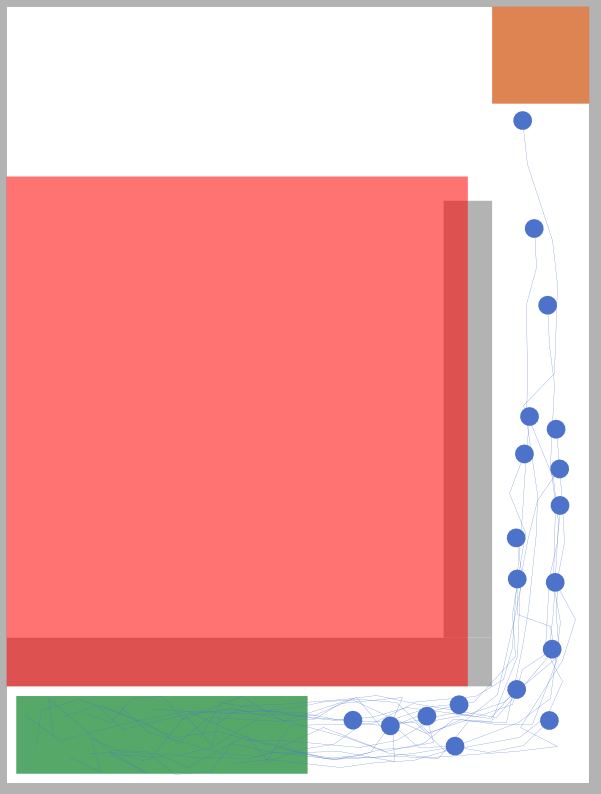
\includegraphics[width=0.7\textwidth]{pictures/osm/rimeatest6.png}
        \caption{RiMEA scenario 6 with OSM}
        \label{fig:rimea6_osm}
    \end{figure}
    \item "Chicken Test" scenario: \\
    At first some of the pedestrians do not pass by the obstacle left or right. They walk some steps in the wrong direction in direction of the obstacle and wait until the the most pedestrians have passed the obstacle. Afterwards they turn around and go back on the right path and reach the target as well. This behaviour is caused by the big crowd. In our simulation we did not have such a behaviour. The reason for this could be that we set less pedestrians in our chickentest scenario, so that every pedestrian can reach the target on its own path and is not blocked by any other pedestrian. Our simulation could probably not handle the big amount of pedestrians which vadere uses to simulate the scenario. This scenario was pre-configured as well. In Figure \ref{fig:chickentest_osm} the pedestrians which first take the wrong path and do not pass by the obstacle at the first try can be seen.
    \begin{figure}[H]
        \centering
        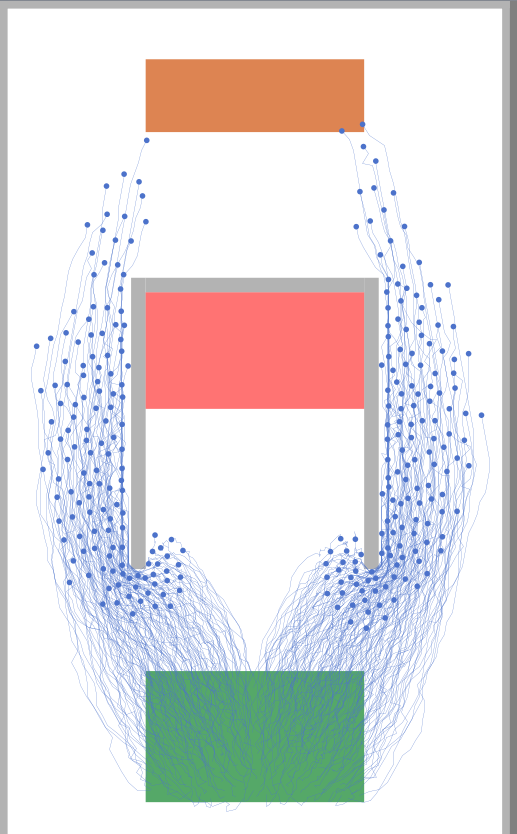
\includegraphics[width=0.7\textwidth]{pictures/osm/chickentest.png}
        \caption{Chickentest with OSM}
        \label{fig:chickentest_osm}
    \end{figure}
    \item General differences and observations: \\
    In general our cellular automoton passes the tests as well as the vadere simulation does. Furthermore, the GUI of vadere lets the user adjust much more things of the simulation. We use the command line to set up different scenarios and adjust them, but we do not offer as many options as vadere does. One example is that the user can set up a mean, minimum, maximum and standard deviation of the pedestrian speed. In our case the pedestrians have a constant speed.
\end{itemize}
\end{task}
\begin{task}{2, Simulation of the scenario with a different model}
For this task we used the same scenarios (RiMEA scenario 1, RiMEA scenario 6 and chickentest scenario) but with different models. Here we use the Social Force Model (SFM) and the Gradient Navigation Model (GNM) and compare them between eahch other.\\
At first the Social Force Model is used to simulate the three scenarios.
\begin{itemize}
    \item RiMEA Scenario 1:\\
    We use the same configurations as for the OSM model. In comparison to the OSM model there cannot be seen any differences. The pedestrian takes 30 seconds to reach the target, which is exactly the same time as the pedestrian needs with the Optimal Steps Model. In Figure \ref{fig:rimea1_sfm} can be seen how the pedestrian walked from the source to the target. Besides, it shows that the pedestrian walks slightly up and down on its path as it does with the OSM.
    \begin{figure}[H]
        \centering
        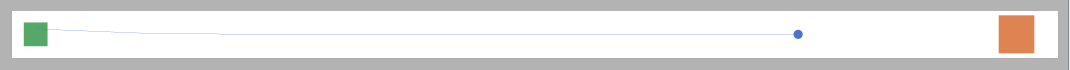
\includegraphics[width=0.7\textwidth]{pictures/sfm/rimeatest1.png}
        \caption{RiMEA scenario 1 with SFM}
        \label{fig:rimea1_sfm}
    \end{figure}
    \item RiMEA Scenario 6:\\
    The RiMEA scenario runs smoother with SFM than the OSM. The distance between the single pedestrians is smaller than for the OSM. The following table containing all pedestrians and the time they take to reach the target, shows that the pedestrians reach faster the target than in the OSM. The reason for that might be that the distance between the pedestrians is smaller.
    \bigbreak
    \begin{tabular}{c|c}
    pedestrianID&evacuationTime\\
         1&  12.0\\
         2& 23.4\\
         3&14.8\\
         4&18.4\\
         5&20.8\\
         6&14.0\\
         7&12.0\\
         8&19.6\\
         9&15.6\\
         10&18.0\\
         11&12.4\\
         12&18.8\\
         13&18.8\\
         14&13.6\\
         15&16.0\\
         16&14.0\\
         17&22.0\\
         18&14.8\\
         19&23.6\\
         20&13.2\\
    \end{tabular}
    \bigbreak
    Figure \ref{fig:rimea6_sfm} shows that the distance between the pedestrians is smaller than before. It can be seen from that picture that the radius with which the pedestrians walk around the corner is smaller for the SFM than for the OSM. Figure \ref{fig:rimea6_sfm2} shows the corner situation and makes it clearer that all the pedestrians have less distance towards each other.
    \begin{figure}[H]
        \centering
        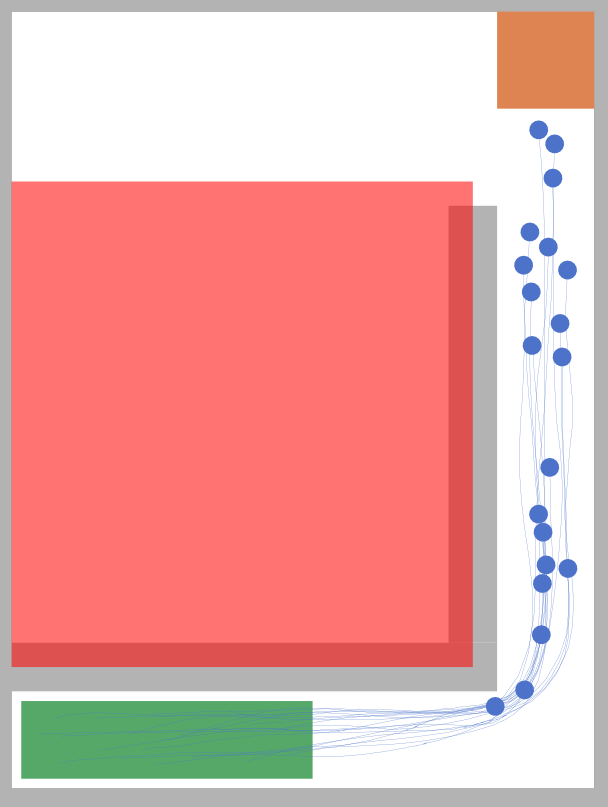
\includegraphics[width=0.7\textwidth]{pictures/sfm/rimeatest6.png}
        \caption{RiMEA 6 scenario with SFM}
        \label{fig:rimea6_sfm}
    \end{figure}
    \begin{figure}[H]
        \centering
        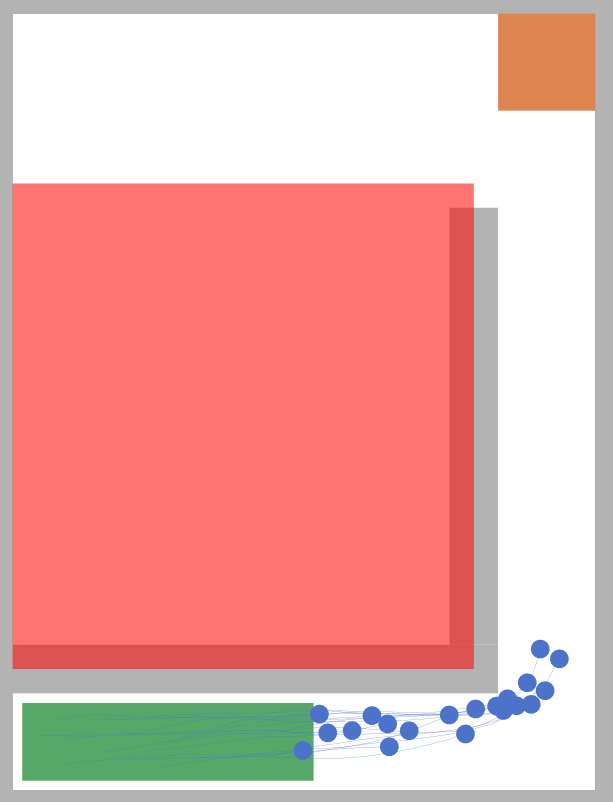
\includegraphics[width=0.7\textwidth]{pictures/sfm/rimeatest6_atcorner.png}
        \caption{RiMEA scenario showing the corner with SFM}
        \label{fig:rimea6_sfm2}
    \end{figure}
    \item Chickentest:\\
    The number of pedestrians is set to 300 to make it possible to compare the OSM to the SFM. If the Social Force Model is used the pedestrians try not not to avoid other pedestrians as much as for the OSM. Consequently, less people leave the right path and walk in the wrong direction towards the obstacle. So less people get stuck for a while in the region of the obstacle, even though we observed a problem that some pedestrians overlap with the obstacle and jump over it. Figure \ref{fig:chickentest_sfm} shows that much less pedestrians get stuck at the inner side of the obstacle than before. Furthermore it shows the encountered problem that pedestrians jump over the obstacle. This can be seen from the paths leading over the obstacle.
    \begin{figure}[H]
        \centering
        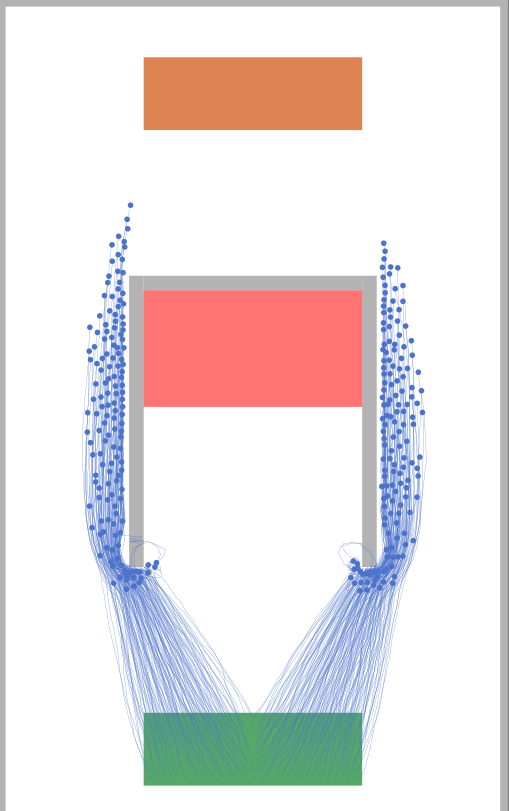
\includegraphics[width=0.7\textwidth]{pictures/sfm/chicken.png}
        \caption{Chickentest with SFM}
        \label{fig:chickentest_sfm}
    \end{figure}
\end{itemize}
After using the Social Force Model for simulating the three scenarios and comparing the results to the results from OSM the Gradient Navigation Model is used in the following paragraph.
\begin{itemize}
    \item RiMEA 1 Scenario:\\
    There are no differences to the other models. The pedestrian takes 30 seconds to reach the target as for the other two models as well. Figure \ref{fig:rimea1_gnm} shows that the pedestrian walks as for the previous models slightly not straight which supports our claim that the shape of the cells of the grid is responsible for that, since the model cannot be responsible for this.
    \begin{figure}[H]
        \centering
        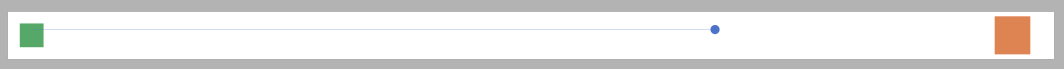
\includegraphics[width=0.7\textwidth]{pictures/gnm/rimeatest1.png}
        \caption{RiMEA scenario 1 with GNM}
        \label{fig:rimea1_gnm}
    \end{figure}
    \item RiMEA Scenario 6:\\
    The difference to the previous models is that the pedestrians try to walk along the wall around the corner. So they are stick at the wall. This behaviour can be seen in Figure \ref{fig:rimea6_gnm}. In comparison to the previous models it seems unnaturally.
    \begin{figure}[H]
        \centering
        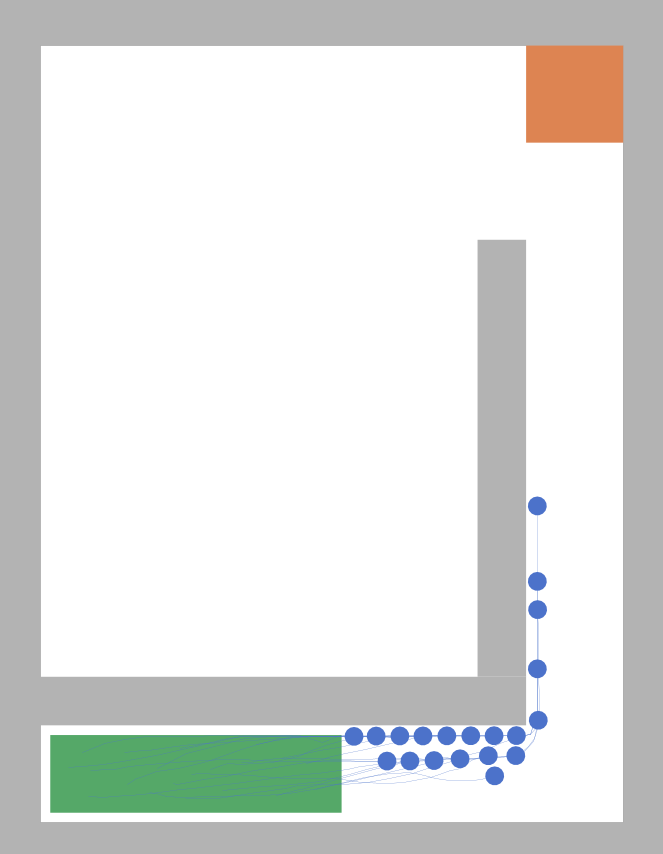
\includegraphics[width=0.7\textwidth]{pictures/gnm/rimeatest6.png}
        \caption{RiMEA scenario 6 with GNM}
        \label{fig:rimea6_gnm}
    \end{figure}
    \item Chickentest:\\
    For the GNM model simulated with the chickentest scenario the pedestrians gather a lot at the corners of the obstacle, but do not enter the area surrounded by the obstacle. This is different to the other used models. Besides, the problem of the SFM does not occur anymore here. There are no pedestrians which jump over the obstacle from the inner side of the obstacle to the outer side of the obstacle. Furthermore the pedestrians take some more time to reach the target because they do not walk with a big radius around the obstacle. They try to pass by slightly the obstacle and walk very close to it. Another remarkable difference is that the computational work for the GNM is heavy. It takes more compuational work than for the OSM and SFM. The phenomen that the pedestrians gather at the corners of the obstacle and slightly walk around the corner can be seen in Figure \ref{fig:chickentest_gnm}.
    \begin{figure}[H]
        \centering
        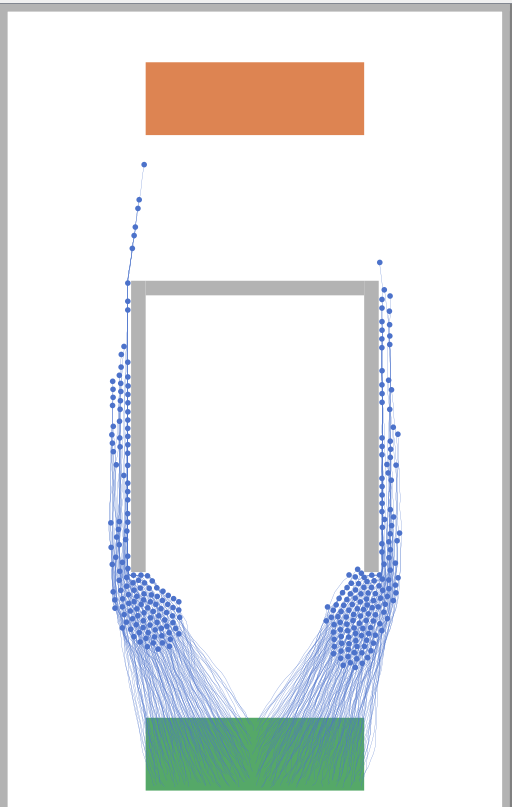
\includegraphics[width=0.7\textwidth]{pictures/gnm/chicken.png}
        \caption{Chickentest with GMN}
        \label{fig:chickentest_gnm}
    \end{figure}
\end{itemize}

\end{task}

\begin{task}{3, Interaction of pedestrians}
The new pedestrian needs only 9.6 seconds to reach the target since it starts walking at the corner. We set up the pedestrian at the position (12.3, 1.8) with the targetId of 1. We used the json library of Python to read the scenario file of the “Corner Scenario” and adjusted it so that the additional pedestrian is added to the corner at position (12.3,1.8). We gave the newly generated JSON file’s path as an argument on the command line and ran Vadere from the console as well. The output can be seen below where the first column is the pedestrian ID and the second column is the arrival time at the target. The pedestrian of ID 1 is the one that was added to the corner.\\
\bigbreak
    \begin{tabular}{c|c}
    pedestrianID&evacuationTime\\
        1&	9.6\\
        2&	22.8\\
        3&	15.6\\
        4&	14\\
        5&	12.\\
        6&	19.6\\
        7&	22\\
        8&	16.4\\
        9&	14.4\\
        10&	21.6\\
        11&	17.2\\
        12&	14.8\\
        13&	18.4\\
        14&	13.2\\
        15&	11.2\\
        16&	19.6\\
        17&	26\\
        18&	14.8\\
        19&	20.4\\
    \end{tabular}
    \bigbreak
\end{task}
\begin{task}{4, Obstacle avoidance}

3. The entropy increases logarithmically as the \texttt{model\_error} parameter increases (see Figure \ref{fig:entropy_change_task4}). Since \hat{M} has a linear relationship with \texttt{model\_error} and \hat{M} is fed in into the logarithm function to calculate the entropy, the entropy shows a logarithmic correlation with \texttt{model\_error}. Thus, the bigger the model error, the more the model differs from the truth; but the rate of difference diminishes. 

\begin{figure}[H]
    \centering
    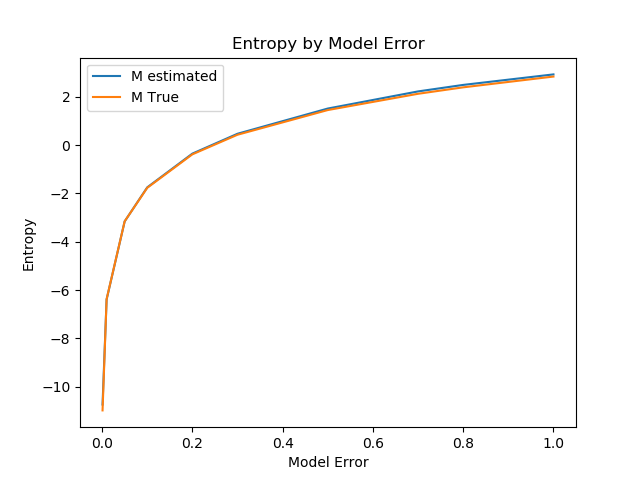
\includegraphics[width=0.7\textwidth]{pictures/task4_entropy.png}
    \caption{Change of entropy by model error}
    \label{fig:entropy_change_task4}
\end{figure}

\end{task}
\begin{task}{5, Tests}
\begin{enumerate}
\item[TEST1:] RiMEA scenario 1 (straight line, ignore premovement time)\\
- not done, but citing RiMEA guideli -
\item[TEST2:] RiMEA scenario 4 (fundamental diagram, be careful with periodic boundary conditions).\\
- test successful - 
\item[TEST3:] RiMEA scenario 6 (movement around a corner).\\
- test successful - 
\item[TEST4:] RiMEA scenario\\
- test successful - 
\end{enumerate}
\end{task}

\bibliographystyle{plain}
\bibliography{Literature}

\end{document}